\documentclass[11pt]{article}
\usepackage{amsmath, amsfonts, amsthm, amssymb}  % Some math symbols
\usepackage{enumerate}
\usepackage{fullpage}

\usepackage[x11names, rgb]{xcolor}
\usepackage{tikz}
\usepackage[colorlinks=true, urlcolor=blue]{hyperref}
\usepackage{graphicx}
\usetikzlibrary{snakes,arrows,shapes}

\usepackage{listings}
\usepackage{array}
\usepackage{mathtools}
\setlength{\parindent}{0pt}
\setlength{\parskip}{5pt plus 1pt}
\pagestyle{empty}

\def\indented#1{\list{}{}\item[]}
\let\indented=\endlist

\newcounter{questionCounter}
\newenvironment{question}[2][\arabic{questionCounter}]{%
    \addtocounter{questionCounter}{1}%
    \setcounter{partCounter}{0}%
    \vspace{.25in} \hrule \vspace{0.5em}%
        \noindent{\bf #2}%
    \vspace{0.8em} \hrule \vspace{.10in}%
}{}

\newcounter{partCounter}[questionCounter]
\renewenvironment{part}[1][\alph{partCounter}]{%
    \addtocounter{partCounter}{1}%
    \vspace{.10in}%
    \begin{indented}%
       {\bf (#1)} %
}{\end{indented}}

%%%%%%%%%%%%%%%%% Identifying Information %%%%%%%%%%%%%%%%%
%% This is here, so that you can make your homework look %%
%% pretty when you compile it.                           %%
%%%%%%%%%%%%%%%%%%%%%%%%%%%%%%%%%%%%%%%%%%%%%%%%%%%%%%%%%%%
\newcommand{\myhwname}{Homework 2}
\newcommand{\mysection}{CS Fundamentals: Scratch Review [due Tuesday]}
%%%%%%%%%%%%%%%%%%%%%%%%%%%%%%%%%%%%%%%%%%%%%%%%%%%%%%%%%%%
\begin{document}
\begin{center}
    {\Large \myhwname} \\
    \mysection \\
    \today
\end{center}

%%%%%%%%%%%%%%%%% PROBLEM 1: Probability Review %%%%%%%%%%%%%%%%%%%%%%%%%
\section{Review: Doodle Jump Pt. 2 [Expected Duration: 15 - 60 min]}
\textbf{If you have any questions about the directions or any blocks you have not used before, let me know via email or text!}\\
\noindent\makebox[\linewidth]{\rule{\paperwidth}{0.4pt}}\\
Although we will not be working on anything on Sketch for today, I would \textbf{strongly recommend installing the \href{https://scratch.mit.edu/scratch2download/}{offline version of Scratch 2}} for future projects.\\\\
\href{https://youtu.be/ZJAsPQanvtg}{Click this line to see a YouTube video of this game running!}\\\\
In the last lesson, we went over the code that we built together. For homework, I want you to describe what is happening in each block shown below. There will be code labeled. I want you to use the \textbf{word} bank below to complete this assignment. Note that \textbf{the words in the word bank is used exactly once... all words are used}.\\\\
If you have any questions regarding the terms in the word bank, \textbf{please} let me know!\\\\
You may find the preview of the game useful.\\
\begin{center}
  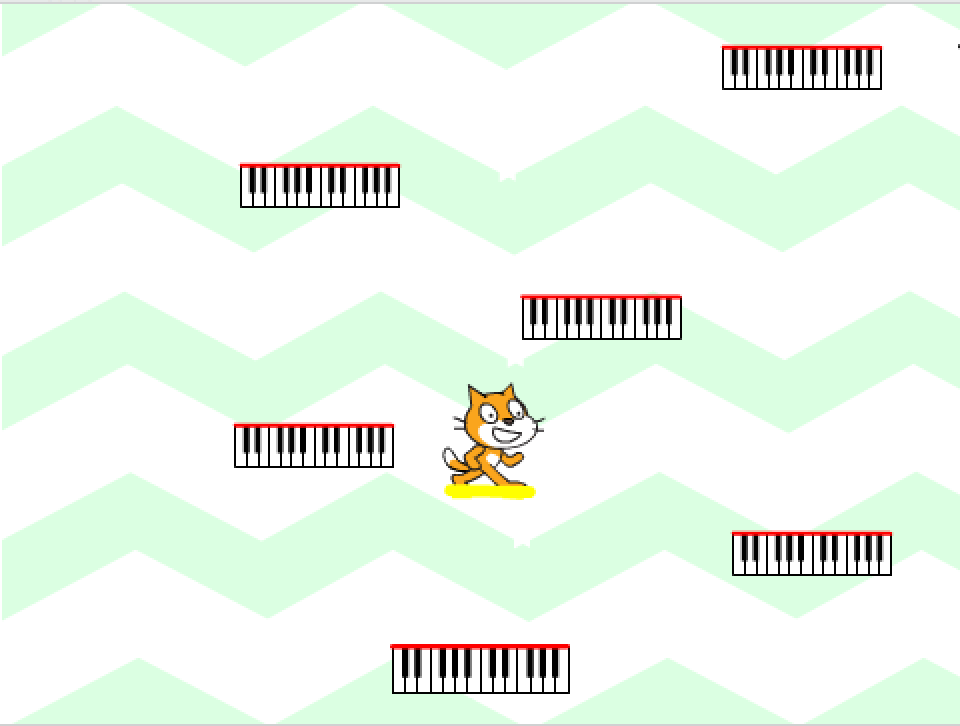
\includegraphics[width=4.5in]{preview.png}
 \end{center}
Do your best and have fun!\\
\noindent\makebox[\linewidth]{\rule{\paperwidth}{0.4pt}}\\
\begin{center}
\textbf{Word Bank:}
\begin{tabular}{|c|c|c|c|}
    \hline
    -180 & 180 & bottom & bottom edge \\
    \hline
    clone & clone & direction & down \\
    \hline
    edge & endless & endless & fall \\
    \hline
    hides & initial & jump & jump \\
    \hline
    key & left & position & red \\
    \hline
    shows & smooth & up & yellow \\
    \hline
\end{tabular}
\end{center}
\noindent\makebox[\linewidth]{\rule{\paperwidth}{0.4pt}}\\
\begin{center}
  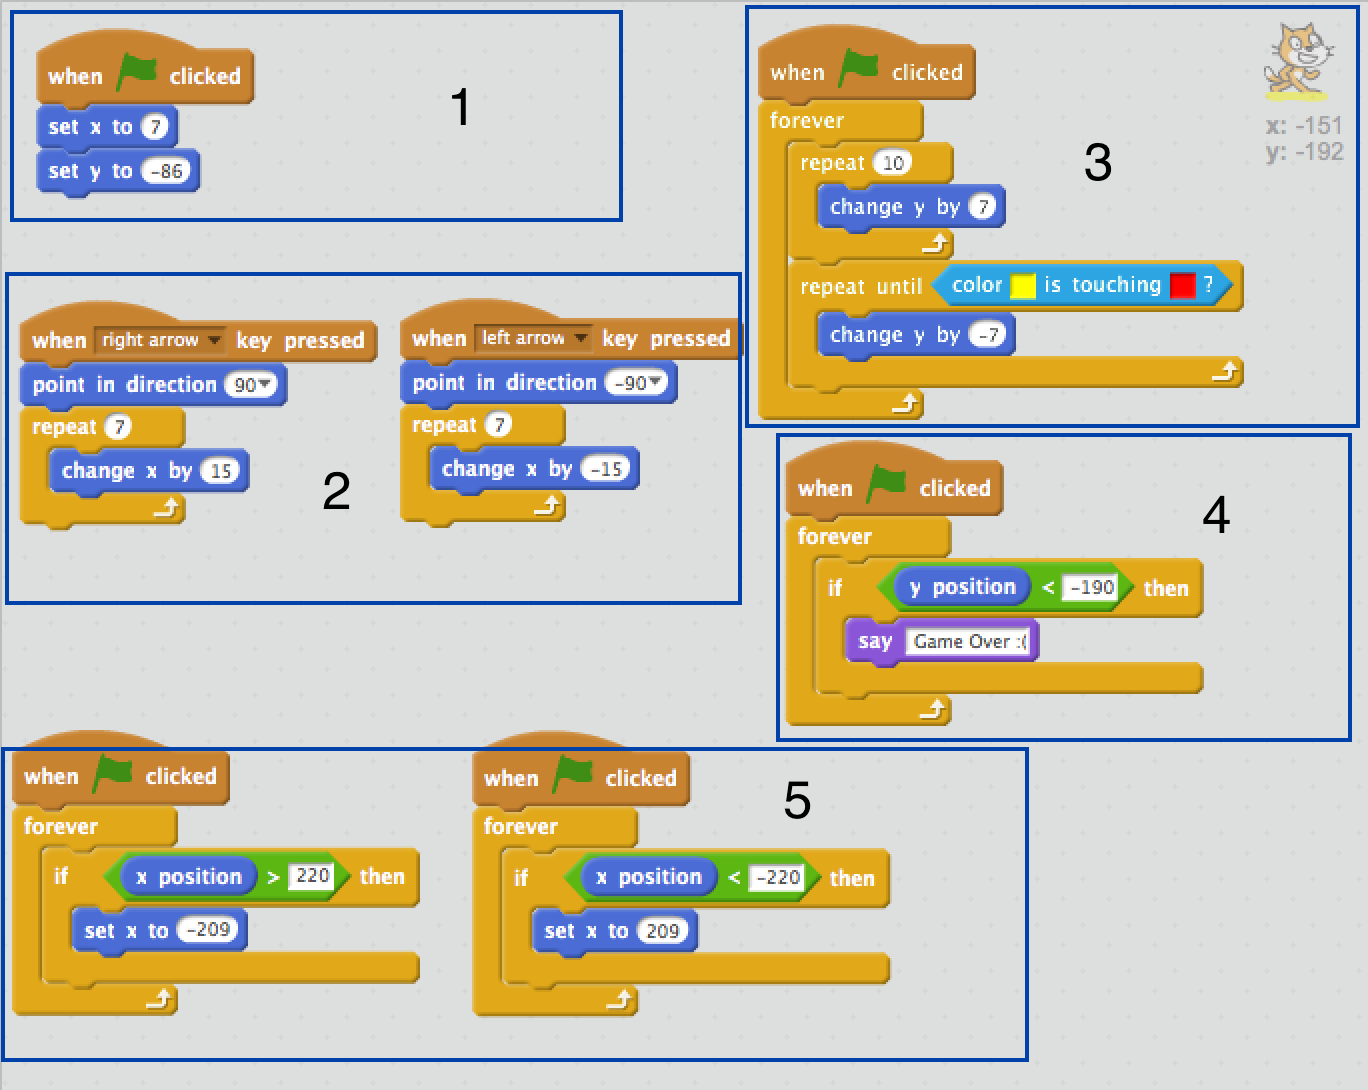
\includegraphics[width=5.5in]{cat.png}
 \end{center}

\begin{enumerate}
\item The Cat
\begin{enumerate}[a.]
\item Block 1 sets the $\rule{2.5cm}{0.15mm}$ position of the Cat.
\item Block 2 changes the $\rule{2.5cm}{0.15mm}$ of the cat based on the $\rule{2.5cm}{0.15mm}$ pressed.
\item In Block 2, we repeat changing the x value 7 times because we want to show a [smooth] transition from one position to another.
\item In Block 3, we loop a few code blocks forever because we want the cat to $\rule{2.5cm}{0.15mm}$ forever.
\item In Block 3, where we repeat change y by 7 10 times, the cat is going $\rule{2.5cm}{0.15mm}$.
\item In Block 3, where we repeat change y by -7 until color yellow is touching red, the cat is going $\rule{2.5cm}{0.15mm}$.
\item In Block 3, the ``color yellow is touching red'' is a condition for when the cat's $\rule{2.5cm}{0.15mm}$ feet touching the piano tile's $\rule{2.5cm}{0.15mm}$ top.
\item Block 4 tells the player that the game is over when the Cat touches the $\rule{2.5cm}{0.15mm}$ edge of the screen.
\item Block 5 lets the user go to the $\rule{2.5cm}{0.15mm}$ edge of the screen to appear in the right, and vice versa.
\item In Block 5, we set the x value to 209 instead of around 220 because the cat may end up getting stuck on the $\rule{2.5cm}{0.15mm}$ of the screen.
\end{enumerate}
\end{enumerate}
\noindent\makebox[\linewidth]{\rule{\paperwidth}{0.4pt}}\\
\begin{center}
  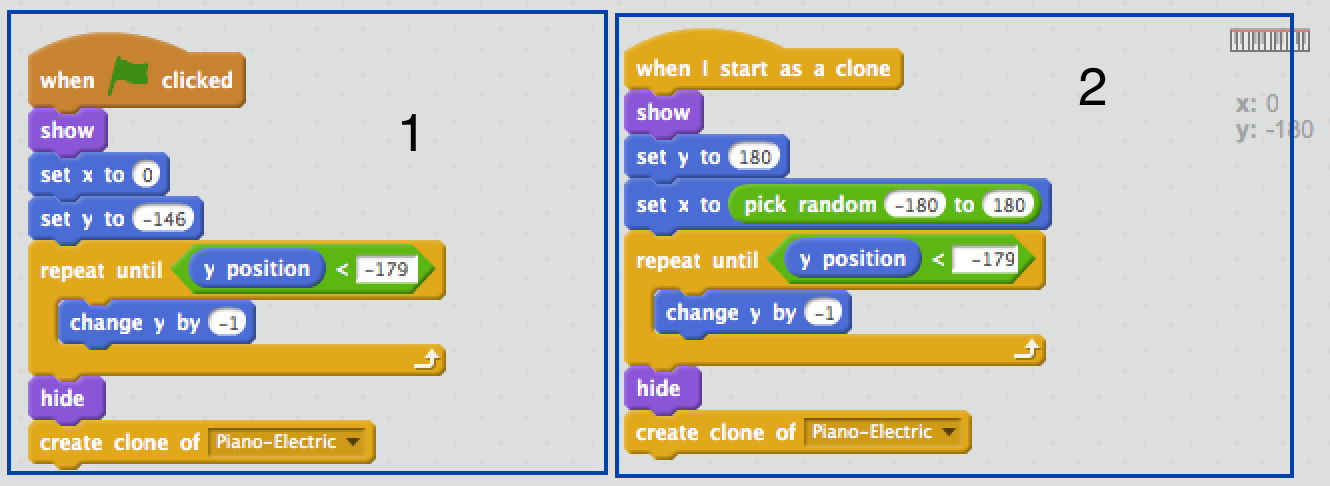
\includegraphics[width=5.5in]{block.png}
 \end{center}
\begin{enumerate}
\item The Tiles
\begin{enumerate}[a.]
\item Block 1 sets the initial $\rule{2.5cm}{0.15mm}$ of the tile, then makes the tile $\rule{2.5cm}{0.15mm}$ until the tile reaches the $\rule{2.5cm}{0.15mm}$ of the screen, then $\rule{2.5cm}{0.15mm}$ the piano tile, and finally creates a $\rule{2.5cm}{0.15mm}$ of the Piano Tile.
\item In Block 1, we hide the piano block so that the cat will no longer be able to $\rule{2.5cm}{0.15mm}$ on the tiles that already hit the bottom of the screen.
\item In Block 1, we create a clone of the Piano Tile so that this game will be $\rule{2.5cm}{0.15mm}$.
\item Block 2 first $\rule{2.5cm}{0.15mm}$ the piano tile, then sets the y position of the piano tile to be at the $\rule{2.5cm}{0.15mm}$ of the screen, then sets the x position of the piano tile to be anywhere between $\rule{2.5cm}{0.15mm}$ to $\rule{2.5cm}{0.15mm}$.
\item At the end of Block 2, we $\rule{2.5cm}{0.15mm}$ the Piano Tile again so that the game will continue to be $\rule{2.5cm}{0.15mm}$.
\end{enumerate}
\end{enumerate}
\end{document}
